\subsection{Experimental Results}\label{subsec:experimental-results}

\subsubsection{Input Workpiece Variation}\label{subsubsec:input-workpiece-variation}

\subsubsection{Pause Duration Variation}\label{subsubsec:pause-duration-variation}

\begin{figure}
    \centering
    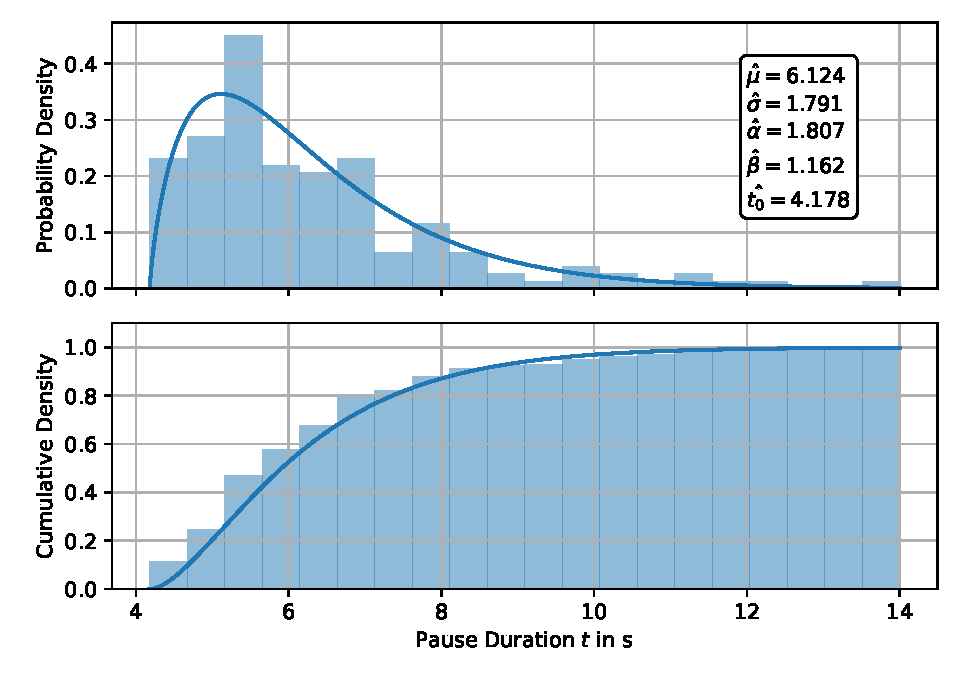
\includegraphics[width=\linewidth]{img/plot_histogram_pauses}
    \caption{Density and Cumulative Histograms of Inter-Pass Durations With Fitted Gamma Distribution}
    \label{fig:plot_histogram_pauses}
\end{figure}

\subsection{Simulation Results}\label{subsec:simulation-results}

In the following, three questions shall be investigated and answered:
\begin{enumerate}
    \item What is the difference in behavior of variations sourced in the input workpiece and arising within the process?
    \item What is the influence of elastic mill response on the variational behavior of the process?
    \item Is there a minimum number of passes needed to eliminate variations of the input workpiece?
\end{enumerate}

For this distinct simulations were carried out and compared with each other and the experimental data.

\subsubsection{Different Sources of Variation}\label{subsubsec:different-sources-of-variation}

Two basic classes of variation sources in can be identified in rolling processes, or manufacturing processes in general: variations inherent to the input workpiece and variations arising in the regarded processes itself.
These effect together the variation of the resulting product.
To investigate the different behavior of them, two simulations shall be carried out and compared.
The first one only regards variations of the input workpiece and how they evolve during the process.
The second one introduces additional variations within the process in means of varying inter-stand pause durations between the reversing passes.
These originate, as denoted before, in the manual handling of the workpiece for feeding into the next pass.
The focus of the following analysis lies on the temperature evolution of the workpiece, since this is crucial for microstructure evolution and final material properties, and will, presumably, be heavily effected by varying pause durations.

\begin{figure}
    \begin{subfigure}{\linewidth}
        \centering
        \includegraphics{img/plot_input_temperature}
        \caption{Under Influence of Input Workpiece Variation}
        \label{fig:plot_input_temperature}
    \end{subfigure}
    \begin{subfigure}{\linewidth}
        \centering
        \includegraphics{img/plot_durations_temperature}
        \caption{Under Influence of Input Workpiece Variation and Pause Duration Variation}
        \label{fig:plot_durations_temperature}
    \end{subfigure}
    \caption{Variation of Workpiece Temperature}
\end{figure}


The temperature evolution of the first case is shown in \autoref{fig:plot_input_temperature}.
The variation of the input workpiece was taken as obtained in \autoref{subsubsec:input-workpiece-variation}.
The box plots in the figure show the variation of the workpiece temperature, where the box marks a distance of $\Estimated\StandardDeviation$ to $\Estimated\Mean$ and the whiskers a distance of $3\Estimated\StandardDeviation$.
The variation of temperature decreases with each processing step and is remarkably small in the product.
So there is something like a ``natural'' depression of variation in each process step.

The second case, however, is shown in \autoref{fig:plot_durations_temperature}.
Here, the variation is not decreasing with each step, but increasing in the transport steps.
In contrast, roll passes still decrease the variation.
If the overall variation decreases in the process, depends, of course, on the ratio between decrease in passes and increase in transports.
In this view, the goal of process design must be to prevent an overall increase of variation in the process.
The main vantage point for this is to limit variation in pause durations.

\begin{figure}
    \centering
    \includegraphics{img/plot_temperature_std}
    \caption{Comparison of Temperature Variation Evolution Between Input Variation and Process Variation}
    \label{fig:plot_temperature_std}
\end{figure}

\autoref{fig:plot_temperature_std} shows the evolution of variation of both cases in comparison.
One can see, that the overall variation is increasing solely in the reversing transport for the second case.
Note, that the influence of transports in oval cross-section shape is remarkably higher than those in round shape.
This can be explained by the adverse surface area to volume ratio of oval cross-sections.

\begin{figure}
    \begin{subfigure}{\linewidth}
        \centering
        \includegraphics{img/plot_input_temperature_correlation}
        \caption{Under Influence of Input Workpiece Variation}
        \label{fig:plot_input_temperature_correlation}
    \end{subfigure}
    \begin{subfigure}{\linewidth}
        \centering
        \includegraphics{img/plot_durations_temperature_correlation}
        \caption{Under Influence of Input Workpiece Variation and Pause Duration Variation}
        \label{fig:plot_durations_temperature_correlation}
    \end{subfigure}
    \caption{Correlation Between Change in Temperature Standard Deviation and Change in Temperature Per Unit}
\end{figure}

From this, the hypothesis that process steps with high influence on temperature have also high influence on the variation depression can be stated.
This is proofed by plotting the relative depression in standard deviation per step as in \autoref{eq:relative-variation-depression} over the change in temperature in the step.
This correlation can especially be observed in varying only the input workpiece as shown in \autoref{fig:plot_input_temperature_correlation}, where the variation depressions in roll passes and transports show an approximately linear correlation to the temperature changes.
In the case of varying pause durations, the roll passes still show the same behavior, but the correlation in the transports is destroyed by the introduction of additional variation, as can be seen in \autoref{fig:plot_durations_temperature_correlation}.

\begin{equation}
    \RelativeStandardDeviationDepression = \frac{\Abs{\Change{\StandardDeviation}}}{\Abs{\StandardDeviation}}
    \label{eq:relative-variation-depression}
\end{equation}

% Vergleich Korngröße

\subsubsection{Elimination of Input Variation}\label{subsubsec:elimination-of-input-variation}

A common statement found is that the variations in the input workpiece are eliminated after three to four passes.
To validate this statement, simulations under different variations of the input workpiece have been carried out.

\autoref{fig:plot_filling_stds} shows the depression of the filling ratio standard deviation along the pass sequence for different initial workpiece diameter variations.
It is found that the variation decreases rapidly in the first three passes and is negligible small in the fourth, no matter what initial variation was applied.
So regarding the geometry the validity of the former statement can be confirmed.

\autoref{fig:plot_temperature_stds}, however, shows the depression of temperature variation along the pass sequence for different initial workpiece temperature variations.
Although, the variation is effectively depressed in the sequence, the variation of the output workpiece is still remarkably higher for higher input variations.
So regarding the temperature evolutions, the statement can not be confirmed, especially in regard of microstructure evolution heavily effected by the temperature path taken.

\begin{figure}
    \begin{subfigure}{\linewidth}
        \centering
        \includegraphics{img/plot_filling_stds}
        \caption{Variation of Roll Pass Filling Ratios}
        \label{fig:plot_filling_stds}
    \end{subfigure}
    \begin{subfigure}{\linewidth}
        \centering
        \includegraphics{img/plot_temperature_stds}
        \caption{Variation of Workpiece Temperature}
        \label{fig:plot_temperature_stds}
    \end{subfigure}
    \caption{Depression of Workpiece Variation}
\end{figure}

% Einfluss auf Mikrostruktur